%; whizzy chapter
% -initex iniptex -latex platex -format platex -bibtex jbibtex -fmt fmt
% 以上 whizzytex を使用する場合の設定。

%     Tokyo Debian Meeting resources
%     Copyright (C) 2011 Junichi Uekawa

%     This program is free software; you can redistribute it and/or modify
%     it under the terms of the GNU General Public License as published by
%     the Free Software Foundation; either version 2 of the License, or
%     (at your option) any later version.

%     This program is distributed in the hope that it will be useful,
%     but WITHOUT ANY WARRANTY; without even the implied warranty of
%     MERCHANTABILITY or FITNESS FOR A PARTICULAR PURPOSE.  See the
%     GNU General Public License for more details.

%     You should have received a copy of the GNU General Public License
%     along with this program; if not, write to the Free Software
%     Foundation, Inc., 51 Franklin St, Fifth Floor, Boston, MA  02110-1301 USA

%  preview (shell-command (concat "evince " (replace-regexp-in-string "tex$" "pdf"(buffer-file-name)) "&"))
% 画像ファイルを処理するためにはebbを利用してboundingboxを作成。
%(shell-command "cd image201101; ebb *.png")

%%ここからヘッダ開始。

\documentclass[mingoth,a4paper]{jsarticle}
\usepackage{monthlyreport}

% 日付を定義する、毎月変わります。
\newcommand{\debmtgyear}{2011}
\newcommand{\debmtgmonth}{1}
\newcommand{\debmtgdate}{15}
% (+ (* (- 2010 2005) 12) 10) started from zero
\newcommand{\debmtgnumber}{72}

\begin{document}

\begin{titlepage}
\thispagestyle{empty}
% タイトルページ:編集必要な部分は最初のマクロに飛ばすこと

\vspace*{-2cm}
第\debmtgnumber{}回 東京エリア Debian 勉強会資料\\
\hspace*{-2cm}
\includegraphics[width=210mm]{image201003/debsen.eps}\\
\hfill{}\debmtgyear{}年\debmtgmonth{}月\debmtgdate{}日

% ここはアップデートすること
\rotatebox{10}{\fontsize{32}{32} {\gt 特集1: キネクト}}

\rotatebox{10}{\fontsize{32}{32} {\gt 特集2: アンケートシステム}}

\vspace*{-2cm}
\hfill{}
\includegraphics[height=6cm]{image200502/openlogo-nd.eps}
\end{titlepage}

\dancersection{Introduction}{上川 純一}

\begin{multicols}{2}
 

 今月のDebian勉強会へようこそ。これからDebianの世界にあしを踏み入れると
 いう方も、すでにどっぷりとつかっているという方も、月に一回Debianについ
 て語りませんか?

 Debian勉強会の目的は下記です。

 \begin{itemize}
 \item \underline{Debian Developer} (開発者)の育成。
 \item 日本語での「\underline{開発に関する情報}」を整理してまとめ、アップデートする。
 \item \underline{場}の提供。
 \begin{itemize}
  \item 普段ばらばらな場所にいる人々が face-to-face で出会える場を提供
	する。
  \item Debian のためになることを語る場を提供する。
  \item Debianについて語る場を提供する。
 \end{itemize}
 \end{itemize}		

 Debianの勉強会ということで究極的には参加者全員がDebian Packageをがりがり
 と作るスーパーハッカーになった姿を妄想しています。情報の共有・活用を通し
 て Debianの今後の能動的な展開への土台として、「場」としての空間を提供す
 るのが目的です。

\end{multicols}

\newpage

\begin{minipage}[b]{0.2\hsize}
 \definecolor{titleback}{gray}{0.9}
 \colorbox{titleback}{\rotatebox{90}{\fontsize{80}{80} {\gt デビアン勉強会} }}
\end{minipage}
\begin{minipage}[b]{0.8\hsize}
\hrule
\vspace{2mm}
\hrule
\begin{multicols}{2}
\tableofcontents
\end{multicols}
\vspace{2mm}
\hrule
\end{minipage}

\dancersection{事前課題}{上川 純一}

今回の事前課題は以下です:
\begin{enumerate}
 \item 2011年の勉強会でなしとげたいことを宣言してください 
 \item 2015年のDebianがどうなっているか大胆に妄想してください。
\end{enumerate}

この課題に対して提出いただいた内容は以下です。
\begin{multicols}{2}
{\small
 %; whizzy-master ../debianmeetingresume201101.tex
% $B0J>e$N@_Dj$r$7$F$$$k$?$a!"$3$N%U%!%$%k$G(B M-x whizzytex $B$9$k$H!"(Bwhizzytex$B$,MxMQ$G$-$^$9!#(B

\begin{prework}{$B>e@n(B $B=c0l(B}

\preworksection{2011$BG/$NJY6/2q$G$J$7$H$2$?$$$3$H$r@k8@$7$F$/$@$5$$(B }

$B:#G/$O(BLAMP $B%9%?%C%/!"(BKVS$B$J$I!"%/%i%&%I%$%s%U%i$r(BDebian$B$G0lDL$j9=C[$9$k;E(B
$BAH$_$r<B8=$9$kJ}K!$K$D$$$F0lDL$jJY6/$7$F4XO"$7$?%Q%C%1!<%8%s%0$K$^$D$o$k(B
$BLdBj$K$D$$$F@0M}$7$?$$!#(B

\preworksection{2015$BG/$N(BDebian$B$,$I$&$J$C$F$$$k$+BgC@$KLQA[$7$F$/$@$5$$!#(B}
 
Debian$B$O$^$@@8$-;D$C$F$$$F!"(BSqueeze+2$B$N%j%j!<%9=`Hw$GK;$7$$!#(B
$B%G%P%$%9$O7HBSEEOC$H%?%V%l%C%H%G%P%$%9$N%5%]!<%H$,DI2C$5$l$F$*$j!"(B
$B%a%$%s%9%H%j!<%`$N(BCPU$B%"!<%-%F%/%A%c$O(Bx86\_64 $B$H(B arm$B!#(B

$B%G%P%C%0MQ$N>pJs$,%G%U%)%k%H$GA4It$N%Q%C%1!<%8$K$D$$$FDs6!$5$l$k!#(B

$BA4(BVCS$B$r6&DL$GMxMQ$G$-$k$h$&$J%$%s%?%U%'!<%9$,@0Hw$5$l!"(B
Debian$B$N%=!<%9%Q%C%1!<%8$rI8=`E*$J(BVCS$B$H$7$FDs6!$5$l$k$h$&$K$J$k!#(B

Debian$B$N%5!<%P%j%=!<%9$O(BP2P$B%*!<%P%l%$%M%C%H%o!<%/7PM3$GDs6!$5$l!"(B
$B6&M-$N%S%k%I%5!<%P$J$I$,MxMQ$G$-$k$h$&$K$J$C$F$$$k!#(B

\end{prework}

\begin{prework}{$B$^$($@$3$&$X$$(B}

\preworksection{2011$BG/$NJY6/2q$G$J$7$H$2$?$$$3$H$r@k8@$7$F$/$@$5$$!#(B}

 $B%9%^!<%H%U%)%s4XO"$N(BWeb$B%"%W%jMQ%i%$%V%i%j$H%M%$%F%#%V%"%W%jJQ49%D!<%k$J(B
 $B$I$N3+H/4D6-$r(BDebian$B$G@0Hw$9$kJ}K!!"2?$,$I$&M%$l$F$$$k$+$rJY6/$7$?$$!#(B
 Debian$B$G4D6-$r@0$($k0Y$K$O$I$l$,(BDebian$B%Q%C%1!<%8(B
 $B$K$J$C$F$$$k$N$+!"$I$l$OBP1~2DG=$G!"$I$l$,IT2DG=$J$N$+!#(BDebian$B>e$G@8@.(B
 $B$7$?%"%W%j$r(BDebian$B$+$iG[?.$9$k!"$"$k$$$O4{B8$NG[?.$N;EAH$_$HO"F0$9$k$?(B
 $B$a$N;EAH$_$O$G$-$J$$$+!#(B

\preworksection{2015$BG/$N(BDebian$B$,$I$&$J$C$F$$$k$+BgC@$KLQA[$7$F$/$@$5$$!#(B}

 $B0U30$H(BWheezy$B$N<!$N%j%j!<%9$,=P$F$7$^$C$F$$$k!#%9%^!<%H%U%)%s8~$1$N%$%s(B
 $B%9%H!<%i$,EP>l$7!"(Bjail break$B$d(Brooted$B$7$J$/$F$b!"4JC1$K(BDebian$B$r%$%s%9%H!<(B
 $B%k$G$-$F$7$^$&!#(BwebOS$B$,(Bipkg$B$r$d$a$F!"(BDebian$B%Q%C%1!<%8$r;H$&$h$&$K@hADJV(B
 $B$j$7$F$$$k(B(webOS$B$K$O5/;`2s@8%[!<%`%i%s$G@8$-;D$C$F$$$F$[$7$$(B)$B!#$=$b$=$b(B
 2015$BG/$K$O%9%^!<%H%U%)%s$H$+%/%i%&%I$H$+$$$&8@MU$O(B $B>C$($F!"$^$?JL$N?7$7(B
 $B$$%P%:%o!<%I$KJQ$o$C$F$$$k$K0c$$$J$$!#(B

\end{prework}


\begin{prework}{ $BF|HfLn(B $B7<(B }

1. Debian$BJY6/2q$N>oO"$K4X?t7?8@8l$N0&9%<T$r0l?M$G$bB?$/A}$d$9!#4X?t7?8@8l$r;H$C$?%O%s%:%*%s$H$+$d$l$?$i3Z$7$=$&!#(B
2. Debian 8.0 $B%j%j!<%9(B?




$BCY$l$FMh$k$+!"$b$7$+$9$k$H=P@J$G$-$J$$$+$b$7$l$^$;$s!#(B

\end{prework}

\begin{prework}{ $B%-%?%O%i(B }

1. 2011$BG/$NJY6/2q$G$J$7$H$2$?$$$3$H$r@k8@$7$F$/$@$5$$(B
$B!!!!!JEl5~%(%j%"$G$N!KJY6/2q$K3'6P!#$b$A$m$sL5CY9o!#(B

2. 2015$BG/$N(BDebian$B$,$I$&$J$C$F$$$k$+BgC@$KLQA[$7$F$/$@$5$$!#(B 
$B!!!!<+$i%+!<%M%k$r:n$k$h$&$K$J$C$F$$$?$j!"(BAT$B%3%s%Q%A$N(BPC$B$r(B
$BHt$S=P$7!">JEENO$d%/%i%9%?Ey$NFCJL$J5!G=$r<B8=$9$k%O!<%I%&%'%"(B
$B%j%U%!%l%s%9$rE83+$7$F$?$j!"%5%]!<%H@AIi2q<R$,=PMh$F$?$j!"(B
$BLQA[$O4v$D$+9M$($?$N$G$9$,!"<B:]$O:#$H$"$^$jJQ$o$i$:C8!9$H(B
$B3+H/$,B3$1$i$l$F$$$k$h$&$K;W$$$^$9!#(B

\end{prework}

\begin{prework}{ henrich }

\preworksection{2011$BG/$NJY6/2q$G$J$7$H$2$?$$$3$H$r@k8@$7$F$/$@$5$$(B }

$B@.$7?k$2$kL\I8$O:#$N$H$3$m$"$j$^$;$s!DB?>/$J$j$H$b;I7c$,<u$1$i$l$l$P$$$$(B
 $B$J!"$H9M$($F$$$^$9!#(B

\preworksection{2015$BG/$N(BDebian$B$,$I$&$J$C$F$$$k$+BgC@$KLQA[$7$F$/$@$5$$!#(B}

Hurd$B$,$D$$$K(B{$B%j%j!<%9$5$l$k(B,$B=*N;@k8@$,=P$5$l$k(B}

\end{prework}

\begin{prework}{ $BB<ED?.?M(B }

\preworksection{2011$BG/$NJY6/2q$G$J$7$H$2$?$$$3$H$r@k8@$7$F$/$@$5$$(B }

 $B%Q%C%1!<%8$X$NM}2r$r?<$a$k!#(BDebian$B$X$N%"%C%W%m!<%I$NN.$l$rCN$k!#(B

\preworksection{2015$BG/$N(BDebian$B$,$I$&$J$C$F$$$k$+BgC@$KLQA[$7$F$/$@$5$$!#(B}

 $B%5!<%PMQ$N%G%#%9%H%j%S%e!<%7%g%s$H8@$C$?$i(BDebian!$B$K$J$C$F$$$k!#(B

\end{prework}



\begin{prework}{ $B;3ED(B }

\preworksection{2011$BG/$NJY6/2q$G$J$7$H$2$?$$$3$H$r@k8@$7$F$/$@$5$$(B }

\begin{itemize}
 \item MiniConf$B$N<B8=!JJY6/2qE*$K:GBg$N%H%T%C%/!)!K(B
 \item $B%Q%C%1!<%8:n@.$N:FJY6/2q$r$7$F!"<+8JN.$r2~$a$k(B
 \item $B<j$,$1$k%Q%C%1!<%8$rA}$d$9!u<+J,$G=q$$$?$N$rG[$C$F$_$k(B
\end{itemize}

\preworksection{2015$BG/$N(BDebian$B$,$I$&$J$C$F$$$k$+BgC@$KLQA[$7$F$/$@$5$$!#(B}

\begin{itemize}
 \item /var/lib/dpkg/available$B$,9T?t49;;$G(B50$BK|9T$rD6$(!J$F$5$9$,$K=E$/$F(Bdpkg$B$,D62~NI$5$l$k!J$H$$$$$J!K!K(B
 \item $B2>A[2=%3%s%F%J$,D6Ia5Z$7$D$D8x<0$ND69b5!G=(Bunionfs$B$,?k$K40@.$7!"(Bapt-get$B$G(Bconflict$B$7$?$iB(J,4t$7$FN>J}$N4D6-$rN>N)$7$D$D(Bbind$BE}9g$G$-$k$h$&$K$J$k!J$H$$$$$J!K(B
 \item $B%U%!%$%k%7%9%F%`$N%9%J%C%W%7%g%C%H!&%?%$%`%^%7%s5!G=$,Ia5Z$7$F!"C/$b(Bsid$B$r;H$&$3$H$K7|G0$r46$8$J$/$J$k!J$H$$$$$J!K(B
\end{itemize}


\end{prework}



\begin{prework}{ $BK\>1(B }

\preworksection{2011$BG/$NJY6/2q$G$J$7$H$2$?$$$3$H$r@k8@$7$F$/$@$5$$(B }

$B$:$$$V$sA0$G$9$,!"0MMj$5$l$?$h$&$J5$$N$9$k(Blibsvm$B$K4X$7$FH/I=$7$?$$$G$9!#(B

\preworksection{2015$BG/$N(BDebian$B$,$I$&$J$C$F$$$k$+BgC@$KLQA[$7$F$/$@$5$$!#(B}

$B$A$g$C$HA[A|$D$+$J$$$G$9$M!#(B


\end{prework}



\begin{prework}{ emasaka }

\preworksection{2011$BG/$NJY6/2q$G$J$7$H$2$?$$$3$H$r@k8@$7$F$/$@$5$$(B }

$B$3$3$OH/I=$H$+$$$&$H$$$$$s$G$7$g$&$+!#(B

\preworksection{2015$BG/$N(BDebian$B$,$I$&$J$C$F$$$k$+BgC@$KLQA[$7$F$/$@$5$$!#(B}

TV$B$,(BCPU$B$P$s$P$s@Q$`$h$&$K$J$C$F!"$=$$$D$r(Bhack$B$7$F(BDebian$B$,F0$$$?$j$9$k$H$9$4$$$G$9$M!#(B

\end{prework}



\begin{prework}{ higashiyama }

\preworksection{2011$BG/$NJY6/2q$G$J$7$H$2$?$$$3$H$r@k8@$7$F$/$@$5$$(B }

$B:#G/$OKh2s;22C$7$F!"$?$@(BDebian$B$r;H$&?M$+$i%9%F%C%W%"%C%W$7$?$$(B

\preworksection{2015$BG/$N(BDebian$B$,$I$&$J$C$F$$$k$+BgC@$KLQA[$7$F$/$@$5$$!#(B}

X$B$,$R$C$=$j$H>C$($F$$$/(B

\end{prework}



\begin{prework}{ yamamoto }

\preworksection{2011$BG/$NJY6/2q$G$J$7$H$2$?$$$3$H$r@k8@$7$F$/$@$5$$(B }

$B:#G/$3$=%O%C%+!<$K$J$k!#(B

\preworksection{2015$BG/$N(BDebian$B$,$I$&$J$C$F$$$k$+BgC@$KLQA[$7$F$/$@$5$$!#(B}

Debian $B$,(B sid $B$@$1$N!"%m!<%j%s%0%j%j!<%9$K$J$C$F$*$j!"(B
stable $B$N%j%j!<%9$OGI@8$N%G%#%9%H%j%S%e!<%7%g%s$KG$$;$F$$$k!#(B

\end{prework}


\begin{prework}{ kmuto }


\preworksection{2011$BG/$NJY6/2q$G$J$7$H$2$?$$$3$H$r@k8@$7$F$/$@$5$$(B }

 $B$^$9$^$9K;$7$$$s$@$1$I!"?t2s$O=P@J$7$?$$!#$^$?9V;U$G$-$k$h$&$J%F!<%^$b:n$l$k$H$$$$$J!#(B

\preworksection{2015$BG/$N(BDebian$B$,$I$&$J$C$F$$$k$+BgC@$KLQA[$7$F$/$@$5$$!#(B}

 $B!J(Bwheezy$B$G$O$J$/!K(Bwheezy+1$B$N%j%j!<%9%(%s%8%K%"%j%s%0Cf!"$@$h$M!)!)(B Debian$B$r(BUbuntu$B$K%^!<%8$9$Y$-$@$H$$$&(BGR$B$r=P$9$+$I$&$+$G(Bdebian-vote$B$,%U%l!<%`$K!#(B

$BEvF|$O(BCAcert assurer$B$N;E;v$r$d$kM=Dj!#(B

\end{prework}



\begin{prework}{ $BLnEg!!5.1Q(B }

\preworksection{2011$BG/$NJY6/2q$G$J$7$H$2$?$$$3$H$r@k8@$7$F$/$@$5$$(B }

 3$B$D$0$i$$$O2?$+H/I=$7$F$_$?$$$H;W$$$^$7$?!#(B

\preworksection{2015$BG/$N(BDebian$B$,$I$&$J$C$F$$$k$+BgC@$KLQA[$7$F$/$@$5$$!#(B}

\begin{enumerate}
 \item  Oracle Client $B%i%$%V%i%j$N%5%]!<%H(BOS$B%j%9%H$K(BDebian stable$B$,F~$C$F$$$k!JK\Ev$KM_$7$$(B...)
 \item  X.org$B0J30$N(BWindow System$B$,I8=`:NMQ$K$J$C$F$$$k!#(B
 \item  $B5/F02hLL(B(grub/gdm)$B$d!"%m%0%$%s%a%K%e!<$,%U%k%"%K%a!<%7%g%s$7$F$*$j!"BT5!>uBV$G$OIaDL$K(BBGM$B$,LD$C$F$$$k!#!J%2!<%`$N%a%K%e!<2hLL$_$?$$$J6E$C$?1i=P$,I8=`(B)
 \item  $BDL>o$N%b%K%?$O(B3D$B%b%K%?$GMxMQ$5$l$F$*$j!"(Bkinect$B$N$h$&$J?HBN$r;H$C$FA`:n$9$k$h$&$J%G%P%$%9$,F~NO%G%P%$%9$H$7$FI8=`BP1~!#(B
 \item  Blue-Ray Disk4$BKgAH$_$NG[I[$H$J$k!#(B
 \item  Mysql$B$,(Bupstream$B$N:G?7HG$HF1Ey$H$J$k!#(B
\end{enumerate}

\end{prework}




}
\end{multicols}

\dancersection{最近のDebian関連のミーティング報告}{上川純一}
\subsection{東京エリアDebian勉強会71回目報告}

% (query-replace-regexp "<.*?>" "")
% (query-replace-regexp "^[	 ]\+" "")

東京エリアDebian勉強会。
2010年12月の勉強会が荻窪にて開催されました。
参加者は、松鵜さん、前田さん、
山田(泰)さん、山本浩之さん、yyuuさん、野島さん、
やまねさん、岩松さん、あらきやすひろさん、
野首さん、本庄さん、吉田@板橋さん、上川の14人でした。

2010年を振り返り、2011年にむけてやりたいことを提案しました。2010年12月分
のプレゼン資料PDF にまとめてありますのであとでご覧ください。

本庄さんがlibsaneについて紹介しました。感想として、Debianでlibsaneのコー
ド書くの、簡単じゃん!  簡単なりにいろいろとハマりどころがあったようで、プ
レゼンテーションの軽妙な中身とともに楽しませていただきました。

山田さんがKinectのハック進捗について簡単に紹介しました。来月までにはおもしろいデモができるそうです。

山田さんがCACertの認証について必要なことについて紹介しました。CACertでの
Assurance(認証)を行うにはAssurerにより必要な内容が多数あるようで、大変そ
うでした。2011年1月は実際に認証をしてみようということになりました。

Debian勉強会アンケートシステムの稼働開始と案内について。まぁ当日回答いた
だいた内容についてはシステムがまだまともにう動いていなかったようです先月
回答全然もらえなかったのでまともにデバッグできてなかったよう。これは鋭意
改善中。


\dancersection{Debian Trivia Quiz}{上川 純一}

ところで、みなさん Debian 関連の話題においついていますか?Debian関連の話
題はメーリングリストをよんでいると追跡できます。ただよんでいるだけではは
りあいがないので、理解度のテストをします。特に一人だけでは意味がわからな
いところもあるかも知れません。みんなで一緒に読んでみましょう。

今回の出題範囲は\url{debian-devel-announce@lists.debian.org} や \url{debian-devel@lists.debian.org}に投稿された
内容とDebian Project Newsからです。

\begin{multicols}{2}
 %; whizzy-master ../debianmeetingresume201101.tex
% $B0J>e$N@_Dj$r$7$F$$$k$?$a!"$3$N%U%!%$%k$G(B M-x whizzytex $B$9$k$H!"(Bwhizzytex$B$,MxMQ$G$-$^$9!#(B
%
% $B$A$J$_$K!"%/%$%:$OJL%V%i%s%A$G:n@.$7!"$N$A$K%^!<%8$7$^$9!#5U$K%^!<%8$7(B
% $B$J$$$h$&$K$7$^$7$g$&!#(B
% (shell-command "git checkout quiz-prepare")

\santaku
{RC$B%P%0$N8=>u$O$O$I$3$G3NG'$G$-$k$+(B}
{\url{http://bugs.debian.org/release-critical/}}
{\url{http://localhost/}}
{\url{http://debianmeeting.appspot.com/}}
{A}

\santaku
{Debian$BJY6/2qM=Ls%7%9%F%`$N(BURL$B$O$I$l$+(B}
{\url{http://www.2ch.net/}}
{\url{http://atnd.org/events/}}
{\url{http://debianmeeting.appspot.com/}}
{C}

\santaku
{events@debian.org$B$O$I$3$HE}9g$5$l$?$+(B}
{merchants@debian.org}
{hoge@debian.org}
{fuga@debin.org}
{A}

\santaku
{antiharassment@debian.org $B$N$&$i$K$$$J$$$N$OC/$+(B}
{Amaya Rodrigo Sastre}
{Patty Langasek}
{Kouhei Maeda}
{C}

\santaku
{Sprint$B$G$O$J$$$N$O$I$l$+(B}
{-www sprint}
{security sprint}
{tokyo sprint}
{C}

\santaku
{DACA$B$O$I$3$r8+$l$P$h$$$+(B}
{\url{http://qa.debian.org/daca/}}
{\url{http://daca.debian.org/}}
{\url{file:/tmp}}
{A}

\santaku
{DEP $B$O2?$NN,$+(B}
{Debian Enhancement Proposal}
{Device Enhancement Protocol}
{$B$G$C$W(B}
{A}

\santaku
{DEP5$B$GDs0F$5$l$F$$$k(Bdebian/copyright$B$N5!3#2DFI7A<0$O$I$&$$$&$b$N$+(B}
{S$B<0(B}
{RFC822$BIw(B}
{XML}
{B}


\end{multicols}

%-------------------------------------------------------------------------------
\dancersection{Debian勉強会予約システムにアンケート追加}{上川 純一}
%-------------------------------------------------------------------------------
\index{あんけーと@アンケート}
\index{Debianべんきょうかいよやくしすてむ@Debian勉強会予約システム}

\subsection{アンケートシステムの目的}

Debian勉強会は各自のブログに記述するということが当初事後課題として機能し
ていました。勉強会を開催したあと、参加者は勉強会で得られた内容を整理すること
ができて、開催者は内容がどのようにうけとられたのかをある程度推し量ること
ができました。

しかし、近年勉強会の感想がブログに記述される率が低下してきています
\cite{deb201012annualreport}。原因を想像するに、最近はコミュニケーション
の道具としてのtwitterの流行などにともない、ブログに記述するという習慣が減っ
てきているからなのかもしれません。

時代の変遷によりブログエントリーがなくなるとその機能を代替するものは何で
しょう。

ブログの機能としては、フィードバックのシステムと、あとその他のユーザに勉
強会の記録を伝えるという面がありました。記録の面はtwitterのログをまとめ
るtogetterをなどを使えばよいだろうということが2010年12月の勉強会で提案さ
れ、それで問題は解決しそうです。
残る課題はフィードバックシステムとしての機能です。

勉強会へのフィードバックシステムとしてアンケートシステムを提案します。


\begin{figure}[t]

\begin{minipage}{0.4\hsize}
 \begin{center}
  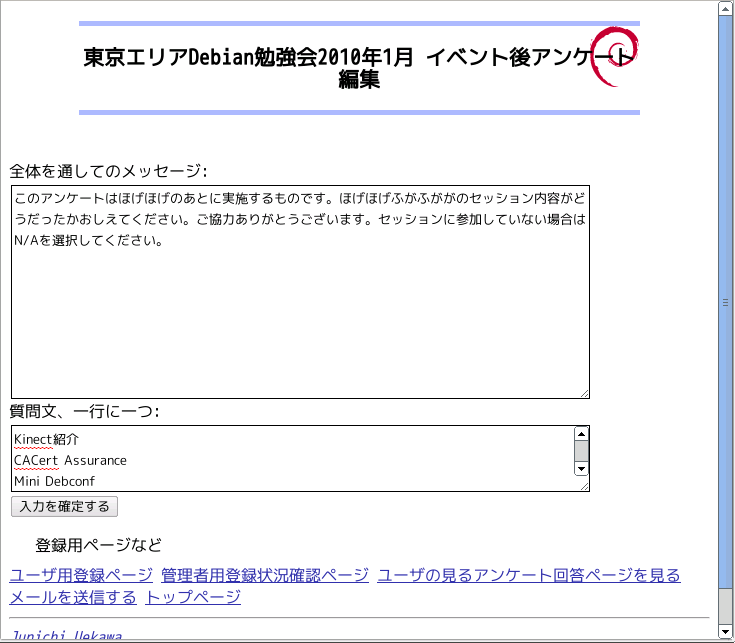
\includegraphics[width=1\hsize]{image201101/enquete-edit.png}
  \caption{アンケート編集画面} 
 \end{center}
\end{minipage}
\begin{minipage}{0.5\hsize}
 \begin{center}
  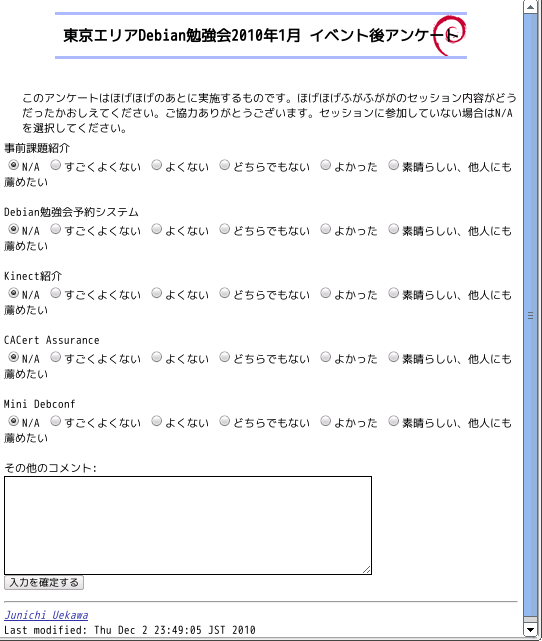
\includegraphics[width=1\hsize]{image201101/enquete-respond.png}
  \caption{アンケート回答画面}
 \end{center}
\end{minipage}
\end{figure}

\subsection{アンケートシステムの利用方法}

\subsubsection{管理者の事前準備}

イベントの管理者はイベントの一覧画面からアンケート作成画面に遷移すること
ができます。そこでは、ユーザに表示するための全体的なメッセージと、各項目
を改行区切りで記述する欄があります。

ユーザにメールを送信すると、ユーザにはリンクの書いてあるメールが届きます。
そのリンクをクリックすると、ユーザはアンケートに回答することができます。

\subsubsection{ユーザ}

ユーザは各項目については0から5までの値で回答することができます。
そして、全体について自由記述の項目があります。
\footnote{勉強会の会場では5択だと中心に回答が偏りがちなので、
4択にしたほうがよいのではないかという意見が出ました。Debian勉強会アンケー
トシステムでは中心に偏り過ぎているとい傾向はまだ出ていないのでこのまま進
めてみようと考えています。}

二つ目的があります。勉強会の企画の中で、どの部分が評価されているのかとい
うのを出していきたいのと、任意なメッセージを入力できるようにすることで会
に対してやりたいことなどの要望が伝えられるようにすることです。

\begin{table}[h]
 \caption{アンケート回答結果の内部表現}
 \begin{itemize}
  \item[0.] N/A \footnote{ユーザにとって回答に値しない、例えば自分がプレゼンテーション
	    していた場合や、遅刻・早退して自分がその場にいなかった、など、ア
	    ンケートに回答できない理由はいろいろありえます。}
  \item[1.] すごくよくない
  \item[2.] よくない
  \item[3.] どちらでもない
  \item[4.] よかった
  \item[5.] 素晴らしい、他人にも薦めたい
 \end{itemize}
\end{table}

\subsubsection{管理者が事後に確認}

管理者は、アンケートの[アンケート集計CSV]リンクをたどることにより、イベ
ント単位のデータのCSVダンプを見ることができます。

特に集計処理はしていません。ここから先はCSVをとりだして処理することにな
ります。

ここで、アンケートが匿名であるべきか記名であるべきかを最初考えていません
でした。どちらがどういう効果があるのかよくわかっていないので今後の課題と
したいと思います。ブログ代わりなのであれば記名でよいと思うのですが、アン
ケートが記名だとバイアスがかかるというのであれば匿名のほうがよいかもしれ
ません。システム的には今は匿名として扱っています。\footnote{Debian勉強会
の会場での議論では、回答の匿名性については。参加者のアンケート回答は匿名
扱いにしたほうが答えにバイアスがかかりにくいだろうという意見が出ました。}

\subsection{アンケートシステムの設計と実装}
\index{Google App Engine SDK}

アンケートシステムの設計と実装について見てみましょう。アンケートはDebian
勉強会予約システム\cite{deb201002debianreserve}の一機能として実装していま
す。

\subsubsection{データストア}

ここの設計で悩んだ点は、EventEnqueteResponseをAttendanceと一緒にするべき
かどうかです。Datastore がjoinをサポートしていないためです。今回は分離し
て必要なときに手動でjoin\footnote{同じキーで二回別のテーブルをqueryするこ
とになるので必要なときには効率が悪いけど、あまり必要にならないと予想した
設計}するアプローチにしてみました。

\begin{commandline}
class EventEnquete(db.Model):
    """Enquete questions for an event."""
    eventid = db.StringProperty()
    overall_message = db.TextProperty()
    question_text = db.StringListProperty()
    timestamp = db.DateTimeProperty(auto_now_add=True)

class EventEnqueteResponse(db.Model):
    """Enquete respnose for an event by one person."""
    eventid = db.StringProperty()
    # responses for 1-5 questions. 0 is N/A
    question_response = db.ListProperty(long)
    overall_comment = db.TextProperty() # a general comment from user.
    timestamp = db.DateTimeProperty(auto_now_add=True)
    user = db.UserProperty()
\end{commandline}

\subsubsection{ユーザインタフェース}

ユーザインタフェース部分は enquete.py に記述しています。メールやHTMLファ
イルの表示部分には、Django のテンプレートを利用しています。

\begin{itemize}
 \item EnqueteAdminEdit.html 管理者用のアンケート編集画面
 \item EnqueteAdminSendMail.txt 管理者が参加者にアンケートを依頼するメー
       ル送信するときのメールのテンプレート
 \item EnqueteAdminShowEnqueteResult.txt アンケートの結果をCSV形式で表示
       する。
 \item EnqueteRespond.html 参加者がアンケートを返答する際に表示される
       HTML。
 \item EnqueteRespondDone.txt 参加者がアンケートを回答したときに送信され
       る確認メール。
\end{itemize}

\subsubsection{バックグラウンドタスク}

ウェブインタフェースからアンケートの送信リクエストがあった場合、
クリックした瞬間にメールの送信処理が発生するわけではなく、
メールの送信処理にtaskqueueを利用しています。

送信元は noreply@debianmeeting.appspotmail.com を使っています。多分ログイ
ンユーザの権限でメールを出すということができないのだと想定してこうなって
います\footnote{未確認}。

\subsection{先月のアンケート集計結果}
\index{R}

それでは、例として2010年12月のアンケート結果をみてみましょう。
0は欠損値なので、Rに処理させる場合は「NA」として処理します。
これでRで処理した結果を見てみましょう。
まだこの時点ではデータが少ないので、今回のなかでどのセッションが
比較的ポジティブな感想を集めたのかということが分かるだけです。

事前準備として、統計解析ツールR\cite{r2008}をインストールします。ここでは
基本パッケージのr-baseとドキュメントのr-doc-info\footnote{R ではなにかわ
からないことがあればとりあえずinfoを見るか、help()コマンドをつかえばよい
かんじです。}をインストールしています。\index{r-base} \index{r-doc-info}

\begin{commandline}
# apt-get install r-base r-doc-info
\end{commandline}
\index{r-base}

R を起動してCSVファイルをロードして、まず基本的な統計量を調べます。

\begin{commandline}
$ R
[中略]
> enquete <- read.csv('201012enquete.csv')
> summary(enquete)
  事前課題紹介  X2010年のDebianを振り返って.2011年を企画する
 Min.   :3.00   Min.   :3                                   
 1st Qu.:3.75   1st Qu.:3                                   
 Median :4.00   Median :4                                   
 Mean   :3.75   Mean   :4                                   
 3rd Qu.:4.00   3rd Qu.:5                                   
 Max.   :4.00   Max.   :5                                   
 NA's   :1.00   NA's   :1                                   
 CACertの準備に何が必要か 俺のlibsaneが火をふくぜ Debian.Miniconf.企画
 Min.   :4.000            Min.   :4.000           Min.   :1.000       
 1st Qu.:4.000            1st Qu.:4.500           1st Qu.:2.000       
 Median :5.000            Median :5.000           Median :3.000       
 Mean   :4.556            Mean   :4.714           Mean   :2.778       
 3rd Qu.:5.000            3rd Qu.:5.000           3rd Qu.:4.000       
 Max.   :5.000            Max.   :5.000           Max.   :4.000       
                          NA's   :2.000                               
> quantile(enquete$俺の, na.rm=TRUE)
  0%  25%  50%  75% 100% 
 4.0  4.5  5.0  5.0  5.0 
> quantile(enquete$Debian)
  0%  25%  50%  75% 100% 
   1    2    3    4    4 
\end{commandline}

ざっと数字を眺めただけですが、今回特に評価の高かったセッションはsaneネ
タと、CACertネタで、評価の低かったセッションはDebian Miniconf企画ネタでし
た。今回のアンケートの結果を受けると、Debian miniconfについてはプレゼンテー
ションの方法を考え直した方がよいだろうと思います。事前課題資料が無かった、
プレゼンテーションしようとしたマシンがプロジェクタにうまくつながらなかっ
た、そもそも話の内容もあまり練られていなかったということを考えるとそれが
そのままアンケートの統計値にも反映したと考えられます。

一つ目線を変えて相関を調べてみました。
しかし、まだこれをどう判断するべきか考えがまとまっていません。

\begin{commandline}
> cor(enquete$CAC, enquete$俺の, use="complete.obs")
[1] 0.7302967
> cor(enquete$俺の, enquete$事前, use="complete.obs")
[1] -0.2581989
> cor(enquete$CAC, enquete$事前, use="complete.obs")
[1] 0
\end{commandline}

また、勉強会で議論した結果出てきた懸念点としては、点数のフィードバックは
毎回出てこられても講師のやる気がそがれるなどの悪影響がある可能性がある点
でした。講師には一年に一回程度まとめて返すのがよいだろうという提案があり
ました。

\begin{thebibliography}{0}
 \bibitem{deb201012annualreport} 上川純一, 「2010年の東京エリアDebian勉強会をふりかえって」
東京エリアDebian勉強会 Deb専 2010年12月号
 \bibitem{deb201002debianreserve} 上川純一, 「東京エリアDebian勉強会予約システムの構想」
東京エリアDebian勉強会 Deb専 2010年2月号
\bibitem{r2008} R Development Core Team, ``R: A Language and
	Environment for Statistical Computing'', R Foundation for
	Statistical Computing, Vienna, Austria, 2008 
	\url{http://www.R-project.org}
\end{thebibliography}

%-------------------------------------------------------------------------------
\dancersection{KinectをDebianで使ってみた}{山田 泰資}
%-------------------------------------------------------------------------------

\index{kinect}
\subsection{Kinectって何?}

KinectはMicrosoftが2010/11にXBox360の新しい操作デバイスとして発売した
ゲームデバイスで、強力な画像認識機能を持ち、一切コントローラなどを
手にしないゲームプレイを実現します。

ハードウェアとしての最大の特徴は、画像認識と言っても単なるカメラではなく、
深度センサを搭載していることです。この種の深度センサ付カメラは従来も
あったのですが、Kinectは大量生産されることもあって価格が1万4千円前後と
従来と比べてまさに桁違いの安さで、このためPCなどの周辺機器として
流用できないかと発売前から高い注目を集めました。

\subsection{発売、そしてKinectハックへ}

そして発売されると普通にUSB接続ができることが判明(単品販売品のみ。
XBox360同梱版はケーブルを加工する必要あり)し、すかさず画像・深度
データのキャプチャ方法が解析されます。こうしてまず生まれたのが
libfreenectです。libfreenectは急速に開発が進み、
\begin{enumerate}
\item カメラ(通常、深度、赤外線)画像の取得
\item カメラのチルト制御
\item 加速度センサの読み出し
\item 筐体LEDの制御
\end{enumerate}
とサウンド関係以外はほぼ制御できるようになり、各種言語へのラッパーが
作られたりOpenCVなどの既成の画像認識ライブラリと組み合わせてデモが
作成されるなど、あっというまに普及が進みました。ここまでが発売後
1ヶ月程の話になります。

しかし、libfreenectだけでは限界がありました。XBox360ではkinectを
使ったゼスチャ認識などの高度な機能を持ったアプリケーション(ゲーム)を
作成できる環境が用意されているのですが、libfreenectはあくまで
ハードウェアにアクセスするまでなので、その部分が欠けていたのです。

実は前評判では「本体側の負荷を下げるため、Kinect側でジェスチャ認識などの
高水準認識も分担する能力がある」という話もあったのですが、最終的には
深度センサまでがハードウェアで、残りはXBox360向けのソフトウェア
ライブラリで実現する形となっていたのでした。

しかし、ここで新展開が起こります。Kinectの深度センサと上記ライブラリの
原型提供を行ったPrimeSense社から、
\begin{enumerate}
\item Linux, Windows用のKinect搭載センサ用ドライバをOSSとして公開する
\item ゼスチャ認識機能を備えた OpenNI フレームワークをOSSとして公開する
\item 骨格認識および高度なジェスチャ認識を行う NITE ライブラリを無償提供する
\footnote{OSSではなく、無償利用のためのライセンスコードが公開された}
\end{enumerate}
という発表が行われ、純正のXBox360開発環境と遜色がなくなり、人気が
さらに高まりました。

これを生かして年末にかけては3Dモデリングツール(MikuMikuDance)に
モーションキャプチャエンジンとして組み込んだり、年明けにはARウルトラ
セブン(画面中の自分の姿にウルトラセブンのコスプレをオーバレイし、
ジェスチャにあわせて様々な必殺技を繰り出すことができる)が登場するなど、
日本では現在進行形で爆発的な盛り上がりを見せています。

ここではOpenNIおよびNITEの利用方法を紹介しつつ、それを元に
Debian勉強会のプレゼンテーションをジェスチャで行う支援ツールの
作成までを紹介します。

\subsection{OpenNIとNITEの導入}
まずはインストールです。
\begin{enumerate}
\item 独自に拡張が始まっているOpenNIとドライバ(SensorKinect)はgithubから
\item NITEはバイナリのためPrimeSense社サイト(http://www.openni.org/)から
\end{enumerate}
それぞれ入手します。

現段階ではバージョンの組み合わせによっては動作しないことがあり、
ここでは以下の組み合わせで導入します:
\begin{enumerate}
\item OpenNI (stable) / https://github.com/OpenNI/OpenNI.git
\item SensorKinect (avin2 version) / https://github.com/avin2/SensorKinect.git
\item NITE-Bin-Ubuntu-x64-1.3.0.17.tar.bz2
\end{enumerate}

いくつかのパッケージを入れるなどビルド環境を整えておく必要は
あります
\footnote{apt-get install gcc python2.6 libusb-1.0-0-dev freeglut3-dev doxygen graphviz あたりで整うかと思います}
が、後は付属のドキュメントの通りに進めればトラブルなく導入できました。

まずはOpenNI本体をインストールします:
\begin{commandline}
$ git-clone https://github.com/OpenNI/OpenNI.git
$ cd OpenNI/Platform/Linux-x86/CreateRedist
$ ./RedistMaker # ビルドおよびインストール用バイナリセットを作ります
...
$ cd ../Redist
$ pwd
/d/src/openni/OpenNI/Platform/Linux-x86/Redist
$ sudo ./install.sh
copying shared libraries...OK
copying executables...OK
copying include files...OK
creating database directory...OK
registering module 'libnimMockNodes.so'...OK
registering module 'libnimCodecs.so'...OK
registering module 'libnimRecorder.so'...OK

*** DONE ***
$
\end{commandline}

次にドライバ(といっても、Linux版のものは単なる共有ライブラリです):
\begin{commandline}
$ git-clone https://github.com/avin2/SensorKinect.git
$ cd SensorKinect/Platform/Linux-x86/CreateRedist
$ ./RedistMaker # ビルドおよびインストール用バイナリセットを作ります
...
$ cd ../Redist
$ pwd
/d/src/openni/SensorKinect/Platform/Linux-x86/Redist
$ sudo ./install.sh
creating config dir /usr/etc/primesense...OK
copying shared libraries...OK
copying executables...OK
registering module 'libXnDeviceSensorV2.so' with OpenNI...OK
registering module 'libXnDeviceFile.so' with OpenNI...OK
copying server config file...OK
setting uid of server...OK
creating server logs dir...OK
installing usb rules...OK

*** DONE ***
$
\end{commandline}

そして最後にNITEのインストールです:
\begin{commandline}
$ tar xf NITE-Bin-Ubuntu-x86-1.3.0.17.tar.bz2 -C /d/src/openni/
$ cd Nite-1.3.0.17
$ sudo ./install.bash -l=0KOIk2JeIBYClPWVnMoRKn5cdY4=
...バイナリを/usr/lib等にコピーした後、サンプルコードをビルドする...
$
\end{commandline}

最後のNITEの導入で指定した「0KOIk2JeIBYClPWVnMoRKn5cdY4=」が
無料利用のための公開ライセンスキーになります。

これらのインストールが終わると
\begin{enumerate}
\item /usr/libにlibnim*.so, libXn*.so, libXnV*.so
\item /usr/include/{ni,nite}に各種ヘッダファイル
\item /usr/binにniReg, niLicenseコマンド(モジュールやライセンスの管理用)
\item /var/lib/niにモジュールやライセンスの管理用XMLファイル
\item /usr/etc/primesenseにOpenNIやモジュールの設定・データファイル
\end{enumerate}
という構成になります。/usr/etc/primesenseはLFS的におかしな位置のため、
/var/lib/ni/modules.xmlから参照しているパス設定を変更の上、/etcに
移動させるとよいかもしれません。
\footnote{OpenNIのパッケージを作成予定ですが、このあたりは検証後直す予定}

あと、サンプルコードを動かせるよう一部ファイルを修正しておきましょう。
NITEを展開した Nite-1.3.0.17/Data/ 下のXMLファイルを以下の内容にします。
ライセンスキーの書き込みと、キャプチャ設定の修正・追加になります。

Sample-Scene.xmlの内容:
\begin{commandline}
<OpenNI>
  <Licenses>
    <License vendor="PrimeSense" key="0KOIk2JeIBYClPWVnMoRKn5cdY4="/>
  </Licenses>
  <Log writeToConsole="true" writeToFile="false">
    <!-- 0 - Verbose, 1 - Info, 2 - Warning, 3 - Error (default) -->
    <LogLevel value="3"/>
    <Masks>
    <Mask name="ALL" on="false"/>
    </Masks>
    <Dumps>
    </Dumps>
  </Log>
  <ProductionNodes>
    <Node type="Depth">
      <Configuration>
        <MapOutputMode xRes="640" yRes="480" FPS="30"/>
        <Mirror on="true"/>
      </Configuration>
    </Node>
    <Node type="Scene" />
  </ProductionNodes>
</OpenNI>
\end{commandline}

Sample-Tracking.xmlの内容:
\begin{commandline}
<OpenNI>
  <Licenses>
    <License vendor="PrimeSense" key="0KOIk2JeIBYClPWVnMoRKn5cdY4="/>
  </Licenses>
  <Log writeToConsole="false" writeToFile="false">
    <!-- 0 - Verbose, 1 - Info, 2 - Warning, 3 - Error (default) -->
    <LogLevel value="3"/>
    <Masks>
    <Mask name="ALL" on="true"/>
    </Masks>
    <Dumps>
    </Dumps>
  </Log>
  <ProductionNodes>
    <Node type="Depth" name="Depth1">
      <Configuration>
      <MapOutputMode xRes="640" yRes="480" FPS="30"/>
      <Mirror on="true"/>
      </Configuration>
    </Node>
    <Node type="Gesture" />
    <Node type="Hands" />
  </ProductionNodes>
</OpenNI>
\end{commandline}

Sample-User.xmlの内容:
\begin{commandline}
<OpenNI>
  <Licenses>
    <License vendor="PrimeSense" key="0KOIk2JeIBYClPWVnMoRKn5cdY4="/>
  </Licenses>
  <Log writeToConsole="true" writeToFile="false">
    <!-- 0 - Verbose, 1 - Info, 2 - Warning, 3 - Error (default) -->
    <LogLevel value="3"/>
    <Masks>
    <Mask name="ALL" on="false"/>
    </Masks>
    <Dumps>
    </Dumps>
  </Log>
  <ProductionNodes>
    <Node type="Depth" name="Depth1">
      <Configuration>
      <MapOutputMode xRes="640" yRes="480" FPS="30"/>
      <Mirror on="true"/>
      </Configuration>
    </Node>
    <Node type="User" />
  </ProductionNodes>
</OpenNI>
\end{commandline}

これらの内容の意味については次項で解説します。

\subsection{Kinectを叩いてみる - OpenNIを使ってみよう}
それではOpenNIから使ってみましょう。
以下はサンプルを少しいじって、深度カメラを叩いて深度情報を
取得し、それをPPM画像の形でダンプするようにしてみたものです。

\begin{commandline}
/*BINFMTCXX: -Wall -I/usr/include/ni -I/usr/include/nite -lOpenNI
 *
 * 深度情報のキャプチャを行い、PGM画像として保存する。
 * カメラからの距離がピクセルの濃淡で表される画像になる。
 *
 */

#include <XnCppWrapper.h>

#define log(...) do { \
        fprintf(stderr, __VA_ARGS__); fprintf(stderr, "\n");    \
    } while (0)

#define die(...) do { \
        fprintf(stderr, __VA_ARGS__); fprintf(stderr, "\n"); exit(1);   \
    } while (0)

// 深度センサが返すデータは深度が16bit値で左上から並んでいるので、
// そのまま16bit PGMとしてダンプすれば画像になる。
void
ppmsave(xn::DepthMetaData& meta, const char *outfile) {
    const XnDepthPixel* pix = meta.Data();

    XnUInt32 xmax = meta.XRes();
    XnUInt32 ymax = meta.YRes();

    // dump 16bit depth data as 16bit PGM
    FILE* out = fopen(outfile, "w+");
    fprintf(out, "P5\n%d %d 65535\n", xmax, ymax);
    fwrite(pix, sizeof(XnDepthPixel), xmax * ymax, out);
    fclose(out);
}

int
main(int argc, char **argv) {
    xn::Context context;
    xn::EnumerationErrors errors;
    xn::DepthGenerator dgen;
    xn::DepthMetaData meta;

    if (argc < 3) {
        die("Usage: %s kinect.xml depth.pgm", argv[0]);
    }

    // XML構成ファイルでの初期化、深度カメラへの参照取得、そしてキャプチャ
    context.InitFromXmlFile(argv[1], &errors);
    context.FindExistingNode(XN_NODE_TYPE_DEPTH, dgen);
    context.WaitOneUpdateAll(dgen);

    // キャプチャデータの取得と保存
    dgen.GetMetaData(meta);
    ppmsave(meta, argv[2]);

    context.Shutdown();
    return 0;
}
\end{commandline}

これを実行すると、
\begin{commandline}
\$ ./camera3d.cc kinect.xml depth.pgm
\end{commandline}
次のように各ピクセルの深さが画像として取れます:
\begin{center}
\includegraphics[height=6cm]{image201101/depth.eps}
\end{center}
正直何がなんだか?という画像ですが、右側にいるのがノートPCを
膝において座っている私です。

ここでの中核部分は以下の3行です。
\begin{commandline}
context.InitFromXmlFile(argv[1], &errors);
context.FindExistingNode(XN_NODE_TYPE_DEPTH, dgen);
context.WaitOneUpdateAll(dgen);
\end{commandline}

OpenNIではシステム中にどのようなデバイスが存在するか、また、
それらの構成(カメラなら解像度など)はどうなるかを外部のXMLで
記述でき、それを元に初期化を行います。コードだけでも書くことは
できるのですが、その場合は構成を変更するとコードの書き換えが
必要になります。

このコンテキスト(context)を作成し、そこにデバイスやフィルタ(未登場
ですが、センサデータの入力を受けてゼスチャ認識を行い、登録されている
フックをトリガするものなどがあります)といったOpenNIモジュール群を
接続する、というのがOpenNI/NITEのプログラムフローになります。

最後に、上で利用したkinect.xmlも引用しておきます:
\begin{commandline}
<OpenNI>
  <!-- ログ設定。以下の設定で標準出力は使わず Log/*.log に書く -->
  <Log writeToConsole="false" writeToFile="true">
    <LogLevel value="0"/>
    <Masks>
      <Mask name="ALL" on="true"/>
    </Masks>
    <Dumps />
  </Log>

  <ProductionNodes>
    <Node type="Image" name="Kin2D">
      <Configuration>
        <MapOutputMode xRes="640" yRes="480" FPS="30"/>
        <Mirror on="true"/>
      </Configuration>
    </Node>

    <Node type="Depth" name="Kin3D">
      <Configuration>
        <MapOutputMode xRes="640" yRes="480" FPS="30"/>
        <Mirror on="true"/>
      </Configuration>
    </Node>

    <Node type="Scene" />
    <Node type="User" />
    <Node type="Gesture" />
    <Node type="Hands" />
  </ProductionNodes>
</OpenNI>
\end{commandline}
以後の例もすべてこのXMLを使って動かしています。

\subsection{ジェスチャの検出方法 - NITEを使う}
それでは次はジェスチャの認識をさせてみましょう。
こちらではNITEライブラリを利用します。

これもOpenNIフレームワーク上のプログラミングなのでコンテキストを
生成する点は同じですが、NITEではコンテキストを介した深度センサ
データのやりとりのような低レベルの操作は隠され、
\begin{enumerate}
\item ジェスチャー操作の流れを管理する、コンテキストをラップするセッションマネージャ
\item セッションマネージャに登録される各種のジェスチャー検出器
\item それら検出器に登録される、操作検知時に呼び出されるコールバック
\end{enumerate}
という構造のコードになります。操作中・操作終了をセッションマネージャが
判定し、「セッション中」の動作のみが検出器にかかるよう調整しています。

実際にどのようなものになるか、見てみましょう:
\begin{commandline}
/*BINFMTCXX: -Wall -I/usr/include/ni -I/usr/include/nite -lXnVNite -lOpenNI
 *
 * 簡単なジェスチャ認識のテスト。
 * 手を振ってセッション開始すると、プッシュとスワイプ動作を認識する。
 *
 */

#include <XnCppWrapper.h>
#include <XnVNite.h>

/**********************************************************************
 * Utility Functions
 **********************************************************************/

#define log(...) do {                       \
        fprintf(stderr, __VA_ARGS__);       \
        fprintf(stderr, "\n");              \
    } while (0)

#define die(...) do {                       \
        fprintf(stderr, __VA_ARGS__);       \
        fprintf(stderr, "\n");              \
        exit(1);                            \
    } while (0)

/**********************************************************************
 * セッションマネージャや検出器に登録するコールバック関数
 * 現在は個々のジェスチャーを認識した等のログを出すのみ。
 **********************************************************************/

static void
OnSessionStart(const XnPoint3D &p, void *data) {
    log("session start");
}

static void
OnSessionEnd(void *data) {
    log("session end");
}

static void
OnFocusStartDetected(const XnChar *focus,
                     const XnPoint3D &p, XnFloat progress, void *data) {
    log("focus start");
}

static void
OnSwipe(XnVDirection dir, XnFloat speed, XnFloat angle, void *data) {
    log("swipe detected. dir=%d, speed=%f, angle=%f", dir, speed, angle);
}

static void
OnPush(XnFloat speed, XnFloat angle, void *data) {
    log("push detected. speed=%f, angle=%f", speed, angle);
}

/**********************************************************************
 * Main
 **********************************************************************/

int
main(int argc, char **argv) {
    xn::Context context;

    if (argc < 2) {
        die("Usage: %s kinect.xml", argv[0]);
    }

    context.InitFromXmlFile(argv[1]);

    // セッションマネージャと各種検出器の生成
    XnVSessionManager* sm = new XnVSessionManager;
    XnVSwipeDetector*  sd = new XnVSwipeDetector;
    XnVPushDetector*   pd = new XnVPushDetector;

    // セッションマネージャの初期化
    //
    // 手を振って(Wave)セッションに入り、休止状態からのセッション再開は
    // 手を上げる(RaiseHand)。セッション中は下で登録された検出器が操作を
    // 検出するようユーザの動きをそれらに伝達する。
    sm->Initialize(&context, "Wave", "RaiseHand");
    sm->RegisterSession(NULL,
                        OnSessionStart, OnSessionEnd, OnFocusStartDetected);

    // ジェスチャー検出器と検知した際のコールバックを登録
    sm->AddListener(sd);
    sm->AddListener(pd);
    sd->RegisterSwipe(NULL, OnSwipe);
    pd->RegisterPush(NULL, OnPush);

    // 後はずっと入力を待ってはイベント処理するループ
    context.StartGeneratingAll();
    for (;;) {
        context.WaitAndUpdateAll();
        sm->Update(&context);
    }
    return 0;
}
\end{commandline}

最初の深度データの画像を保存する例よりも簡単になりました。
上では XnVSwipeDetector と XnVPushDetector の2種類だけを使いましたが、
NITEには10を超える様々な基本ジェスチャーの検出器があり、また、
複数のジェスチャーを組み合わせた操作に対応するための複合処理などを
行う補助クラスも用意されています。

このように、多種多様な検出器を用意して、煩雑な体の各部の動きの
トラッキングや照合の手間をNITEは省いてくれます。

\begin{itembox}[l]{各種の操作と認識率}
なお、動かしてみるとわかりますが、動作によって「きちんと認識される」度が
結構違います。スワイプは「一瞬手を止めて、それからさっと流す」動作なのですが
非常に認識率が悪いです。一方、プッシュ操作はほぼ確実に認識されます。
プッシュ(Push, Click)動作は手振り(Wave)動作と並んで「セッション開始の
シグナル動作(focus gesture)」として実用的とマニュアルに書かれていますが、
よくわかります。快適な操作感のためには結局カスタムの検出器を作成する必要が
ありそうです。
\end{itembox}

\subsection{アプリケーションの制御方法 - XTestの話}
さて、これまでOpenNI, NITEと例を出してきましたが、次はこれで
認識したジェスチャでどう他のアプリケーションを制御するかです。
今回はX11のxtst(XTest)拡張でマウスやキーイベントを送り、それで
(この資料の)プレゼンテーションが行えるようにします。

XTest自体の使い方は以下のようになります。
\begin{commandline}
/*BINFMTCXX:-Wall -lXtst -lX11
 * XTestを使ったキーとマウスの制御テスト
 */

#include <stdio.h>
#include <stdlib.h>
#include <unistd.h>

#include <X11/Xlib.h>
#include <X11/Xutil.h>
#include <X11/extensions/XTest.h>

#define log(...) fprintf(stderr, __VA_ARGS__)
#define die(...) do { fprintf(stderr, __VA_ARGS__); exit(1); } while (0)

enum { DOWN = 1, UP, DOWNUP };

void
sendkey(Display *disp, unsigned int keysym, int mask) {
    unsigned int kc = XKeysymToKeycode(disp, keysym);
    if (mask & DOWN) { XTestFakeKeyEvent(disp, kc, True, CurrentTime); }
    if (mask & UP)   { XTestFakeKeyEvent(disp, kc, False, CurrentTime); }
    XSync(disp, False);
}

int
main(int argc, char **argv) {
    Display *disp;

    if ((disp = XOpenDisplay(NULL)) == NULL) {
        die("Unable to open display\n");
    }

    // キー入力のテスト - とりあえず ls させてみる
    unsigned int key[] = { XK_L, XK_S, XK_Return };
    for (int i = 0; i < (int)(sizeof(key) / sizeof(*key)); i++) {
        sendkey(disp, key[i], DOWNUP);
    }

    // 相対位置移動
    XTestFakeRelativeMotionEvent(disp, -100, -100, CurrentTime);
    XSync(disp, False);
    sleep(3);

    // 絶対位置移動
    XTestFakeMotionEvent(disp, -1, 100, 100, CurrentTime);
    XSync(disp, False);
    sleep(3);

    // XTestのFakeMotionでなぜかXMing上のポインターが動かないので、
    // XWarpPointerを使ってみるテスト・・・これだと動くようだ。
    XWarpPointer(disp, None, None, 0, 0, 0, 0, 200, 200);
    XSync(disp, False);
    sleep(3);

    // Control押しながら右クリックを実行(メニューが出るか確認)
    sendkey(disp, XK_Control_L, DOWN);
    XTestFakeButtonEvent(disp, 3, True,  CurrentTime);
    XTestFakeButtonEvent(disp, 3, False, CurrentTime);
    sendkey(disp, XK_Control_L, UP);
    XSync(disp, False);

    // 終了
    XTestDiscard(disp);
    XCloseDisplay(disp);

    return 0;
}
\end{commandline}

操作したいアプリケーションに合わせて
\begin{enumerate}
\item XTestFakeKeyEvent
\item XTestFakeButtonEvent
\item XTestFakeMotionEvent
\item XTestFakeRelativeMotionEvent
\end{enumerate}
で操作イベントを送りながら、XSyncで同期を取る(ポインタを移動させて
入力、のような操作で、移動が完了してから入力がされるようにする)というのが
基本的な処理になります。

あとはこれを先のOpenNI/NITEのジェスチャ検知をトリガに発行してやれば、
今回のデモは完成になります。

\subsection{デモ}
さて当日うまくいくか・・・

%-------------------------------------------------------------------------------
\dancersection{CACert Assurance}{山田 泰資}
%-------------------------------------------------------------------------------
\index{cacert}

先月のCAcert報告に引き続き、今回はCAcertのassurance会
\footnote{認証会?サイン会?もうGPGと合わせてサイン会でいいか?}
を行うので、その手順をまとめました。

また、手順についてcacert.orgのMLで質問していたところ、
色々と話が転がって、3/4-5のオープンソースカンファレンス(OSC2011
Tokyo/Spring @ 早大)で、関係者が来日の上、CAcertの公式イベントとして
CAcert ATE (Assurer Training Event) を開催できることになりました。
日本初となります。これについても報告&協力募集します。

\subsection{今日の手順}
今日は練習を兼ねたミニサイン会を行います。必要な資材は用意して
あるので、今日参加された方は政府発行の身分証明書があり、cacert.orgに
アカウントがあればポイントを受けられます。

以下、手順:
\begin{enumerate}

\item 認証を受けたい方は、CAP Formに以下の内容をまず記入して下さい
      \index{CAP Form}
\begin{enumerate}
\item 表面は、\bf{\underline{署名およびAssurer用フィールド以外の各欄}}に記入。名前や誕生日はローマ字と西暦で
\item 裏面は、白紙部分に名前(漢字&カタカナ)と和暦での誕生日を補記として記入
\footnote{これは来るOSC2011で外国の方に認証してもらうための手順として策定中の方法です}
\end{enumerate}

\item Assurerは、以下の確認を行って下さい
\begin{enumerate}
\item CCA(CAcert Community Agreement)
\footnote{CAcertに参加するにあたっての遵守事項}
に同意することの口頭確認、および、その旨のチェックボックスにチェックがあること
\item CAP Formの内容がすべて記入されており、また、提示された身分証明書の通りであること
\item 身分証明書が真正であり、内容が以下を満たすこと
\footnote{可能ならば紫外灯などでの偽造チェックや、他の証明書(政府・民間発行は問わない)での追加確認をします}
\begin{enumerate}
\item 誕生日記載の政府発行の物が1つはあること
\item 写真確認できるものが1つはあること
\end{enumerate}
\end{enumerate}

\item 最後に、\bf{\underline{CAP Formに目の前で署名をし}}、そのままAssurerに渡して別れて下さい。署名がないと無効です!

\item Assurerは、以下の追加作業を行って下さい
\begin{enumerate}
\item CAP FormにAssurerとして署名し、それを最低7年間保管する
\item CAP Form記載のメールアドレスを使って http://cacert.org で検索し、各人にポイントを付与する
\end{enumerate}

\end{enumerate}

ポイントが100ptを超えた方、超えそうな方は https://cats.cacert.org/ の
オンライン試験を通しておくと、100pt以上になった時点から他の人を認証できる
ようになります。なお、アクセスにはCAcert発行のクライアント証明書が必要です。

\subsection{CAcert@OSC2011の計画}
元々OSC2011のDebian枠の空き時間でGPGキーサイン兼CAcertサイン会を
企画していましたが、冒頭の通りcacert.orgの方より打診があり、
\begin{quote}
\Large{日本初のCAcert公式トレーニングイベント(ATE Tokyo)}
\end{quote}
を開催できることになりました。

ATE(Assurance Training Event)というのは通常のサイン会とは若干異なり、
主にAssurerになる・なれる人を対象にした、上位Assurer養成(&CAcertの
信頼性向上)のためのサイン会を兼ねたトレーニングイベントです。
\index{ATE}

たまたま期間中に来日するcacert.orgの方(Peter Yuill氏)がおり、
OSC2011の枠も別途確保できたため、日本でのCAcert立ち上げの好機として
緊急で開催決定となりました。

検討中の日程は以下の通りです:
\begin{enumerate}
\item 3/5昼にOSC2011の正式セッションとしてトレーニング講座を実施する(サインも残り時間やブースで実施)
\item その上で、3/5夕刻から追加サイン会を実施する。実施場所・時間は以下の2案で検討中
\begin{enumerate}
\item 近隣の会議スペースや会場の空きスペースでサイン会をする
\item 飲み屋やレストランのスペースを借りて、その中でサイン会をする
\end{enumerate}
\end{enumerate}

OSC2011は17:00に終了なので、サイン会は前者なら17:00-19:00、後者なら
18:00-エンドレス(酔っ払うまで)で考えています。飲み会内開催案は
\begin{quote}
\Large{「酔っ払いそうだが大丈夫か?」「大丈夫だ、問題ない」\footnote{意訳}}
\end{quote}
と、先にサインをするなど手順を工夫すれば、場所や時間の確保問題を
クリアする案としてよいかもという事です(ドイツのATEでもやってみるとか)。

なお、準備のため、特に運営やサインに協力して下さる方を絶賛大募集中です。
現在の準備状況は以下の通り:
\begin{table}[h]
\begin{center}
\begin{tabular}{|r|p{30em}|}
\hline
必要なもの & 準備状況
\\ \hline
当日参加できるAssurerの方 & 未調整(来場者に100pt渡せるとベスト)
\\ \hline
当日参加できる運営の方 & 未調整(Assurer担当と別に、CAP Form確認や引率に数名)
\\ \hline
場外会場の確保 & 未了(隣接の区のスポーツセンタの優先権がある新宿区の人求む)
\\ \hline
事前告知&申込ページの用意 & 未了(wiki.cacert.orgで行う?atnd等を使える?)
\\ \hline
CAP FormやCCAなどの紙資料 & 準備可能(各100部程度なら市の印刷機で激安)
\\ \hline
ATEプレゼンやCCAの翻訳 & 未了(これが次の山か?頑張ります・・・)
\\ \hline
案内チラシ(場所案内など) & 未了(内容が未作成。印刷は可能)
\\ \hline
ブラックライト(Assurer人数分)& 未了(製作計画中)
\\ \hline
プリンタ(紙資料印刷用) & 準備OK(持って行けます)
\\ \hline
プロジェクタ(場外でプレゼンの場合) & 準備OK(持って行けます)
\\ \hline
終了後レポート & 未了(実施レポートをcacert.orgに出すまでが公式イベント、らしい。これはやります)
\\ \hline
\end{tabular}
\end{center}
\end{table}

なお、開催規模ですが、CAcertの方には、「Assurerまたは100pt近い
Assurer見込み」の状態のATE参加者は10名内外、また、その中で150pt達成
済みのExperiencedAssurerは数名だろうという見込みを伝えています。


\cleartooddpage

\vspace*{15cm}
\hrule
\vspace{2mm}

\includegraphics[width=2cm]{image200502/openlogo-nd.eps}
\noindent \Large \bf Debian 勉強会資料\\
\noindent \normalfont \debmtgyear{}年\debmtgmonth{}月\debmtgdate{}日 \hspace{5mm}  初版第1刷発行\\
\noindent \normalfont 東京エリア Debian 勉強会 (編集・印刷・発行)\\
\hrule

\end{document}
